\documentclass[11pt, compress, aspectratio=1610, serif]{beamer}

\usetheme{pl}

\usepackage{booktabs}
\usepackage{minted}
\usepackage{listings}
\usepackage{color}
\usepackage{fancyvrb}
\newcommand{\VerbBar}{|}
\newcommand{\VERB}{\Verb[commandchars=\\\{\}]}
\DefineVerbatimEnvironment{Highlighting}{Verbatim}{commandchars=\\\{\}}
% Add ',fontsize=\small' for more characters per line
\newenvironment{Shaded}{}{}
\newcommand{\KeywordTok}[1]{\textcolor[rgb]{0.00,0.44,0.13}{\textbf{{#1}}}}
\newcommand{\DataTypeTok}[1]{\textcolor[rgb]{0.56,0.13,0.00}{{#1}}}
\newcommand{\DecValTok}[1]{\textcolor[rgb]{0.25,0.63,0.44}{{#1}}}
\newcommand{\BaseNTok}[1]{\textcolor[rgb]{0.25,0.63,0.44}{{#1}}}
\newcommand{\FloatTok}[1]{\textcolor[rgb]{0.25,0.63,0.44}{{#1}}}
\newcommand{\ConstantTok}[1]{\textcolor[rgb]{0.53,0.00,0.00}{{#1}}}
\newcommand{\CharTok}[1]{\textcolor[rgb]{0.25,0.44,0.63}{{#1}}}
\newcommand{\SpecialCharTok}[1]{\textcolor[rgb]{0.25,0.44,0.63}{{#1}}}
\newcommand{\StringTok}[1]{\textcolor[rgb]{0.25,0.44,0.63}{{#1}}}
\newcommand{\VerbatimStringTok}[1]{\textcolor[rgb]{0.25,0.44,0.63}{{#1}}}
\newcommand{\SpecialStringTok}[1]{\textcolor[rgb]{0.73,0.40,0.53}{{#1}}}
\newcommand{\ImportTok}[1]{{#1}}
\newcommand{\CommentTok}[1]{\textcolor[rgb]{0.38,0.63,0.69}{\textit{{#1}}}}
\newcommand{\DocumentationTok}[1]{\textcolor[rgb]{0.73,0.13,0.13}{\textit{{#1}}}}
\newcommand{\AnnotationTok}[1]{\textcolor[rgb]{0.38,0.63,0.69}{\textbf{\textit{{#1}}}}}
\newcommand{\CommentVarTok}[1]{\textcolor[rgb]{0.38,0.63,0.69}{\textbf{\textit{{#1}}}}}
\newcommand{\OtherTok}[1]{\textcolor[rgb]{0.00,0.44,0.13}{{#1}}}
\newcommand{\FunctionTok}[1]{\textcolor[rgb]{0.02,0.16,0.49}{{#1}}}
\newcommand{\VariableTok}[1]{\textcolor[rgb]{0.10,0.09,0.49}{{#1}}}
\newcommand{\ControlFlowTok}[1]{\textcolor[rgb]{0.00,0.44,0.13}{\textbf{{#1}}}}
\newcommand{\OperatorTok}[1]{\textcolor[rgb]{0.40,0.40,0.40}{{#1}}}
\newcommand{\BuiltInTok}[1]{{#1}}
\newcommand{\ExtensionTok}[1]{{#1}}
\newcommand{\PreprocessorTok}[1]{\textcolor[rgb]{0.74,0.48,0.00}{{#1}}}
\newcommand{\AttributeTok}[1]{\textcolor[rgb]{0.49,0.56,0.16}{{#1}}}
\newcommand{\RegionMarkerTok}[1]{{#1}}
\newcommand{\InformationTok}[1]{\textcolor[rgb]{0.38,0.63,0.69}{\textbf{\textit{{#1}}}}}
\newcommand{\WarningTok}[1]{\textcolor[rgb]{0.38,0.63,0.69}{\textbf{\textit{{#1}}}}}
\newcommand{\AlertTok}[1]{\textcolor[rgb]{1.00,0.00,0.00}{\textbf{{#1}}}}
\newcommand{\ErrorTok}[1]{\textcolor[rgb]{1.00,0.00,0.00}{\textbf{{#1}}}}
\newcommand{\NormalTok}[1]{{#1}}

\makeatletter
\def\maxwidth{\ifdim\Gin@nat@width>\linewidth\linewidth\else\Gin@nat@width\fi}
\makeatother

\usepgfplotslibrary{dateplot}

\newcommand{\begincols}{\begin{columns}}
\newcommand{\stopcols}{\end{columns}}

\title{Jmd conversion}
\subtitle{It just works}
\date{\today}
\author{Timothée Poisot}
\institute{LOLOLOL}

\begin{document}

\maketitle

\begin{frame}[fragile]{How to compile}

This is the code we need

\begin{verbatim}
julia -e 'using Weave; weave("slides.Jmd", doctype="pandoc")'
pandoc slides.md -t beamer
  --slide-level 2
  -o slides.tex
  --template ./template/pl.tex
  --highlight-style pygments
latexmk
\end{verbatim}

\end{frame}

\begin{frame}[fragile]{Using packages}

\begin{Shaded}
\begin{Highlighting}[]
\NormalTok{using StatsBase}
\end{Highlighting}
\end{Shaded}

\end{frame}

\begin{frame}[fragile]{Columns}

\begincols
\column{0.3\textwidth}

You can have columns: 4

\column{0.7\textwidth}

\begin{Shaded}
\begin{Highlighting}[]
\NormalTok{n = }\FloatTok{3}
\NormalTok{A = zeros(}\DataTypeTok{Int64}\NormalTok{, (n, n))}
\KeywordTok{for} \NormalTok{i }\KeywordTok{in} \FloatTok{1}\NormalTok{:n}
  \NormalTok{A[i,i] = i}
\KeywordTok{end}
\NormalTok{A}
\end{Highlighting}
\end{Shaded}

\begin{verbatim}
3×3 Array{Int64,2}:
 1  0  0
 0  2  0
 0  0  3
\end{verbatim}

\stopcols

\end{frame}

\section{Some figures}\label{some-figures}

\begin{frame}[fragile]{Figures}

\begincols
\column{0.35\textwidth}

\begin{Shaded}
\begin{Highlighting}[]
\NormalTok{using Plots}
\NormalTok{pgfplots()}
\NormalTok{p1 = plot(rand(}\FloatTok{10}\NormalTok{),}
  \NormalTok{size=(}\FloatTok{250}\NormalTok{,}\FloatTok{200}\NormalTok{),}
  \NormalTok{lab=}\StringTok{""}\NormalTok{)}
\NormalTok{plot!(p1, rand(}\FloatTok{10}\NormalTok{), c=:red);}
\NormalTok{xaxis!(p1, }\StringTok{"Position"}\NormalTok{);}
\NormalTok{yaxis!(p1, }\StringTok{"Random value"}\NormalTok{);}
\NormalTok{savefig(p1, }\StringTok{"figures/test1.tex"}\NormalTok{);}
\end{Highlighting}
\end{Shaded}

\hfill\column{0.55\textwidth}

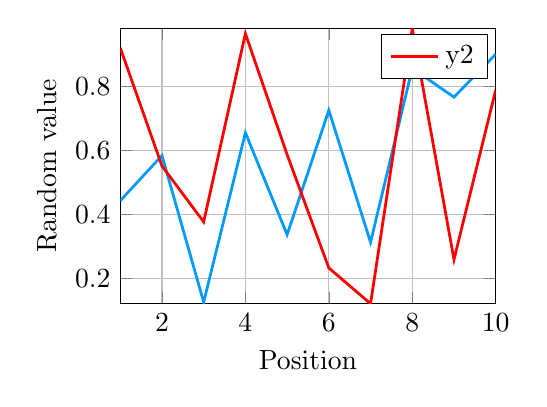
\begin{tikzpicture}[]
\begin{axis}[height = {50.8mm}, ylabel = {Random value}, xmin = {1.0}, xmax = {10.0}, ymax = {0.9821358780550975}, xlabel = {Position}, {unbounded coords=jump, xticklabel style={rotate = 0}, xmajorgrids = true, xtick = {2.0,4.0,6.0,8.0,10.0}, xticklabels = {2,4,6,8,10}, xtick align = inside, yticklabel style={rotate = 0}, ymajorgrids = true, ytick = {0.2,0.4,0.6000000000000001,0.8}, yticklabels = {0.2,0.4,0.6,0.8}, ytick align = inside,     xshift = 0.0mm,
    yshift = 0.0mm,
    axis background/.style={fill={rgb,1:red,1.00000000;green,1.00000000;blue,1.00000000}}
}, ymin = {0.12183275691305706}, width = {63.5mm}]\addplot+ [color = {rgb,1:red,0.00000000;green,0.60560316;blue,0.97868012},
draw opacity=1.0,
line width=1,
solid,mark = none,
mark size = 2.0,
mark options = {
    color = {rgb,1:red,0.00000000;green,0.00000000;blue,0.00000000}, draw opacity = 1.0,
    fill = {rgb,1:red,0.00000000;green,0.60560316;blue,0.97868012}, fill opacity = 1.0,
    line width = 1,
    rotate = 0,
    solid
},forget plot]coordinates {
(1.0, 0.443497676665066)
(2.0, 0.5846085373395244)
(3.0, 0.1267933832036936)
(4.0, 0.6556581846359897)
(5.0, 0.3374149294292428)
(6.0, 0.7257569851673131)
(7.0, 0.3136893202571489)
(8.0, 0.8571002134245078)
(9.0, 0.7669123251437968)
(10.0, 0.9010105138371123)
};
\addplot+ [color = {rgb,1:red,1.00000000;green,0.00000000;blue,0.00000000},
draw opacity=1.0,
line width=1,
solid,mark = none,
mark size = 2.0,
mark options = {
    color = {rgb,1:red,0.00000000;green,0.00000000;blue,0.00000000}, draw opacity = 1.0,
    fill = {rgb,1:red,1.00000000;green,0.00000000;blue,0.00000000}, fill opacity = 1.0,
    line width = 1,
    rotate = 0,
    solid
}]coordinates {
(1.0, 0.9209135545988485)
(2.0, 0.5519101251385714)
(3.0, 0.37738273693000646)
(4.0, 0.9653472674465684)
(5.0, 0.5874374070208361)
(6.0, 0.23342898782043386)
(7.0, 0.12183275691305706)
(8.0, 0.9821358780550975)
(9.0, 0.25994759510271614)
(10.0, 0.789084406638257)
};
\addlegendentry{y2}
\end{axis}

\end{tikzpicture}


\stopcols

\end{frame}

\begin{frame}{Output}

\end{frame}

\section{Some code}\label{some-code}

\end{document}
